\documentclass[10pt]{article}
\usepackage[breaklinks=true]{hyperref}
\usepackage[margin=0.75in]{geometry}

\usepackage{color}
\usepackage{graphicx}
\definecolor{pblue}{rgb}{0.13,0.13,1}
\definecolor{pgreen}{rgb}{0,0.5,0}
\definecolor{pred}{rgb}{0.9,0,0}
\definecolor{pgrey}{rgb}{0.46,0.45,0.48}

\usepackage{listings}
\lstset{language=bash, showspaces=false, showtabs=false,
	breaklines=true, showstringspaces=false, tabsize=2, breakatwhitespace=true,
	commentstyle=\color{pgreen}, keywordstyle=\color{pblue},
	stringstyle=\color{pred}, numbers=left, stepnumber=1,
	basicstyle=\small\ttfamily, frame=single, moredelim=[il][\textcolor{pgrey}]{$$},
	moredelim=[is][\textcolor{pgrey}]{\%\%}{\%\%} }

\title{\textbf{Week 11} \\
\Large Disks, File Systems and the Linux FHS}
\author{ Melvyn Ian Drag }
\date{\today}

\begin{document}
\maketitle

\begin{abstract}
We will explore how physical disks are formatted in Linux,
discuss (some of) your options for formatting your disks, learn about swap
space, and have a look at some of the most important directories that exist on
your Linux machine.
\end{abstract}

\section{Before Class} 
Try to ssh into digital ocean on another port so people
don't need to use their data to get into their servers.


\section{Motivation for Today's lecture}

You might be studying to become any of the following:
\begin{enumerate}
\item Sysadmin
\item Programmer
\item DevOps
\item Network engineer
\item More educated person
\item A power user of your personal laptop
\item Did I miss anything?
\end{enumerate}

In  any one of these situations, you need to be able to add and remove ssds,
usb drives, and hdds from Linux machines. It is somewhat scary to learn how to
do this on your own - it's a good thing you're here today!

\section{Filesytem Hierarcy Standard}

Let's start with the easiest bit. Turn on
your Linux machine and navigate to the root of your filesystem. List the files
and directories there. If you have a laptop and a digital ocean server you might
want to fire both up. If you have a mac, a linux laptop and a server, maybe look
at all three. You will see what they have in common, and what is different.

\begin{lstlisting}
user@machine$ sudo su -
root@machine$ cd / 
root@machine$ ls
# The subject of the coming discussion is here in the stdout.
\end{lstlisting}

\subsection{The important Directories}

{\color{red} \textbf{/}} - root of your Linux install

{\color{red} \textbf{/bin}} - programs needed for single user mode, for bringing
a system up in maintenance mode. I've never had to do this for maintenance, but
the utilities it provides are simple standard commands like `cat`,`ls`, etc.

{\color{red} \textbf{/boot}} - files to be used for booting the system. These
are low level things you won't worry much about as a general desktop user,
application developer, or web programmer. This is lowlevel stuff for getting the
OS up and running between the time you plug it in and hit the power button and
start using Linux. You'll see the Linux kernel, the bootloader (on your system
youll probably see grub, but on an embedded project you'll probably see uboot. )
We'll compile the kernel in this class and maybe poke at the bootloader, but it
might be more instructive to poke at the bootloader of a physical pc sitting in
front of you.

{\color{red} \textbf{/dev}} - devices and things. you'll see your harddrive/sdd
for example as something like /dev/sda. There are a bunch of ttys. What a tty is
and how you use it is of particular interest to me, and maybe during office
hours Ill show you some stuff I do with those devices.

{\color{red} \textbf{/etc}} - config files. We had to edit config files for
apache2 and postgresql before. This is where you find config files for various
applications.

{\color{red} \textbf{/home}} - user home directories. Your homework will be to
put this on a separate physical drive. This is where users put their data.
Photos, downloads, video games, etc.

{\color{red} \textbf{/lib}} - libraries for booting the system and used by
programs on your computer.

{\color{red} \textbf{/lib\textless qual \textgreater}} Youll see 32 and 64 bit
variants of the various libraries. If you don't know what "dynamic" vs. "Static"
linking means, and have never used static vs dynamic libraries, this will be
outside of your understanding.

{\color{red} \textbf{/media}} - where auto mounted media goes. When you stick a
usb stick in, or a CDROM, it will generally appear here.

{\color{red} \textbf{/mnt}} - where you will manually mount filesystems for your
use. We'll explore some use cases of this today.

{\color{red} \textbf{/opt}} - a place for "add on packages". Stuff you want to
install goes here. The use of this directory is debatable and I leave it up to
you to decide what you put here and what philosophical stance you choose on what
ought to go here.

{\color{red} \textbf{/proc}} - we already looked at this when we looked at
stdin/stdout/stderr. We'll revisit that quickly. Write a little python program:

\begin{lstlisting}
import time

while True: 
	time.sleep(10)
	 pass 
\end{lstlisting}

Run it in the back ground

\begin{lstlisting}
user@machine$ python program.py & [outputs pid] 
user@machine$ ls /proc/$pid/fd 0 1 2 
\end{lstlisting}

you see the file descriptors for stdin, stdout, stderr. the /proc has
information about running processes. There is much more to see besides the file
descriptors, but thats the only example I'm going to provide.

{\color{red} \textbf{/root}} - the home direcotry for the root user. The root
user doesn't get a directory in /home.

{\color{red} \textbf{/sbin}} - programs for booting and maintaining the system,
but not used by regular users. 

\begin{enumerate}
\item \url{https://ma.ttias.be/understanding-the-bin-sbin-usr-bin-and-usr-sbin-split/}
\item \url{http://landley.net/writing/hackermonthly-issue022-pg33.pdf}
\end{enumerate}

the difference between sbin and bin has history behind it, and I've linked a few
quick and interesting reads explaining the differences.

Do take a moment to 

\begin{lstlisting}
user@machine$ ls -l /sbin 
\end{lstlisting}

 and notice that many of the commands there are actually links to the commands
in /bin. What's a link? In general it's like a windows shortcut. The actual
program isn't in /sbin, it's in /bin, but when you call the one in /bin, it
calls the one in /sbin. `bash` isn't linked, however, bash is in /bin you'll
see. 

\begin{lstlisting}
$ which bash /bin/bash
$ ls -l /sbin/b*
# bash is not there
\end{lstlisting}

doesn't matter, just showing you.

{\color{red} \textbf{/srv}} - I haven't ever used this. It might be relevant to
you, I don't know

{\color{red} \textbf{/sys}} - don't worry about it

{\color{red} \textbf{/tmp}} - temporary files. Depending on the distro you use
these might or might not be deleted on reboot. They might be cleaned up before
reboot. They are temporary files, and the longevity and uses of them differs and
depends on you.

For example, 

\begin{lstlisting}

ls /tmp
# some stuff about ssh
\end{lstlisting}

that's temporary info about your ssh login. Don't worry about the details. 

{\color{red} \textbf{/usr}} - another location for executables, libraries, etc,
typically read-only stuff that isnt essential to booting the system. There's
alot of argument about what goes in here. If you're a sysadmin or linux
application developer you will work on this.

Notice that tmux isn't essential to your system. 

\begin{lstlisting}
$apt-get install tmux 
$which tmux #/usr/bin/tmux
\end{lstlisting}

If you want to feel confused for a bit, look at this post:

\url{https://unix.stackexchange.com/questions/8656/usr-bin-vs-usr-local-bin-on-linux}

people discuss the uses of /bin, /sbin, /usr/bin, /usr/sbin, /usr/local/bin,
~/bin, etc.

It hasn't mattered to me in my career what goes where, but depending on the
depth you go into Linux you may develop a passionate opinion.

\subsection{Need your help}
Many of you likely have tmux installed already. What
are some other fun packages we can install that will serve for the above
example?

\subsection{Want to learn more?}

There is a popular youtube channel called
'Engineer man' or the like. The videos feature a guy sitting in the lower right
corner of the screen talking about interesting Linux/Programming stuff with his
terminal taking up most of the screen so you can see what stuff he's typing.
There is a good video about the filesystem hierarchy standard.


\section{Drives, Partitions, Mounting, and Partitioning.}

 The idea of this part
of the lecture is that sometimes you want to add storage space to your machine.
You might have a 250GB SDD and you just bought a 1TB drive and you want to add
it to your machine so you can download more movies, save more pictures, store
more code, whatever.

\subsection{Look at what storage space you already have.}

\begin{lstlisting}

$lsblk
sda      disk
--sda1   part 
\end{lstlisting}

sda is a physical drive on your computer, like a harddrive connected to the
machine. sda1 is a partition of the drive, it's a chunk of memory you formatted
in a particular way to become useable by your machine.

\subsection{ Now we will add another drive}
Heres how you do it on digital ocean. the process is the same on your laptop
with a usb stick, ssd, hdd, or whatever persistent storage device you use. We'll
all just use digital ocean to make the experience easy and avoid acidentally
destorying something on the laptop.

Images/addVolume01
Images/addVolume02
Images/addVolume03

Note that there are instructions on digital ocean about how to format. Ignore
that. I'm going to explain how formatting and partitioning work and then you can
go back and see what digital ocean is telling you to do and youll understand and
maybe want to modify what theyve asked you to do.

\begin{lstlisting}
$lsblk
# theres an unpartitioned disk called sda ( or something else! )
\end{lstlisting}

Windows normally gives your drives names like 'C:/', 'D:', 'E:', right? I'm not
a Windows expert but I know that this is what it looks like on a Windows
computer.


\section{What is a Filesystem} 
They are fantastically interesting things. There
are many different types of them. A filesystem is a very lowlevel thing that
described the layout of a physical disk in terms of where the ones and zeros go
on the disk and what they mean when they are in different locations. You will
work mostly with ext3 and ext4 in your life on Linux, but there are others. We
could discuss the differences between them, compare performance of different
file systems, but I feel like that would take away from the flow of this
lecture. 

{\LARGE\textit{Write on board: Do not confuse the Linux filesystem hierarchy (
which we have described above ) with a filesystem, which is more low level
concept of where 1s and 0s are stored on a physical disk.} Some filesystems are
ext3 and ext4, fat. We will use refer to filesystems in this class, you now know
that it is a thing. It is your responsibility to go read about them because we
simply dont have time here and it isn't just a linux concept - it is a computer
concept. Windows, BSD, Linux, etc. all use filesystems.}

\begin{center}
\textbf{After this class, go out and research what ZFS, EXT4,
EXT3, FAT32, etc. are for yourself. It will be enlightening for you as a
computer professional.}
\end{center}

Have a look at the file systems your disks use with:

\begin{lstlisting}
user@machine$ df -TH
\end{lstlisting}


\section{Looking at Partitions, Partitioning and Mounting}

\subsection{Introduction}

Lets look at the two drives we added, the one had a partition on it, the other
one didn't. What does that mean??

lsblk -h shows us options for showing information about our drives. There's alot
to take in. Let's focus on this command:


\subsection{parted}

If you happen to miss class and are reading these notes, here's a good reference
to get you started

\url{https://www.digitalocean.com/community/tutorials/how-to-partition-and-format-storage-devices-in-linux}

These notes ought to be good, but sometimes it helps to have another reference.

You may notice that drive sda is 10G and the partition sda1 takes up the full
10G, whereas sda2 takes up only 4XX GB of the 500GB on the disk, and then sdc is
a 500GB drive with no partition. There are some weird things happening here and
I'm going to explain the basics to you.

We are going to format and add some space to our machine under /mnt, just to do
it as an exercise.

\begin{lstlisting}
# below I refer to /dev/sdc. The added disk will likely have a different name
# like sda or sdb on your machine! Be careful!
sudo parted /dev/sdc mklabel gpt # sdc is the name of hte drive, not a
partition.
sudo parted /dev/sdc mkpart primary ext4 0% 100% # same as above
lsblk
# now its there
sudo mkfs.ext4 /dev/sdc1
sudo mkdir -p /mnt/newdrive
sudo mount /dev/sdc1 /mnt/newdrive
lsblk
# now the partition is mounted
lsblk --output  NAME,FSTYPE,SIZE,MOUNTPOINT
\end{lstlisting} 

You can also unmount the drive

\begin{lstlisting}
# note the command is umount, NOT unmount!
user@machine$ #sudo umount mountpoint
user@machine$ sudo umount /mnt/newdrive
\end{lstlisting}

\subsection{ Again step by step}

\begin{lstlisting}
sudo parted /dev/sdc mklabel gpt
\end{lstlisting}

We first label the disk. This layouts the structure of the disk. There are other
names for the label - partition table and partition map are other names. The
disk has some metadata about the partitions it contains and how they are
structured, that's what this is for. You will mainly be interested in mbr/msdos
or gpt partition tables. There's plenty to be said about mbr vs gpt partition
tables. If you want to leave class knowing something, though maybe not
understanding it fully - MBR is good for drives up to 2TB. Past that you need
GPT. GPT is associated with UEFI whereas MBR is associated with BIOS. If you're
confused, keep studying. In the meantime, just use gpt on Linux.


\begin{lstlisting}
root@machine$ parted -l
# you can look through here to verify that you have labeled your disk as gpt.
# The label is also refered to as a Partition table!
\end{lstlisting}

Now to add a partition to the labeled disk. So far the disk is  not useable
for storage.

\begin{lstlisting}
sudo parted /dev/sdc mkpart primary ext4 0% 100%
\end{lstlisting}

This command puts a partition on the labeled disk. The partition can be
extended/logical or primary. For us we will make a primary partition. We also
tell parted what file system type we are going to put in the partition. We will
use ext4. There are many file system types, and you can read in depth about them
if you're interested. ext4 is "the best file system type in Linux" in some
senses, and not as good as file system types in other senses. It's up to you how
much you want to know. Here's a reference to get you started:

\begin{enumerate}
\item\url{https://opensource.com/article/17/5/introduction-ext4-filesystem}
\item\url{https://askubuntu.com/questions/44908/what-is-the-difference-between-ext3-ext4-from-a-generic-users-perspective}
\end{enumerate}

We also made the partition start at 0\% and go all the way to the end of the
drive.

\begin{lstlisting}
sudo mkfs.ext4 /dev/sdc1 
\end{lstlisting}

This puts the ext4 filesystem on the partition you created. A good question to
ask yourself is "why did we type ext4 in the command to create the partition?"
We'll ignore that question for now and continue on our quest to add some more
disk space to our machines.

\begin{lstlisting}
sudo mkdir -p /mnt/newdrive
\end{lstlisting}

create a mount point for your new disk. You can put it in mnt for now.

\begin{lstlisting}
sudo mount /dev/sdc1 /mnt/newdrive
\end{lstlisting}

Now mount your disk. 

You can see it with 

\begin{lstlisting}
lsblk
\end{lstlisting}

or also with

\begin{lstlisting}
user@machine$ df
\end{lstlisting}

Now mount/unmount the drive a few times to check it out.

Add some stuff to the partition, unmount it, remount it. see stuff is still
there.

unmount it and mount it somewhere else. 

see the stuff you created is still there under the mount point.

\subsection{Restarting machine makes this go away}

\begin{lstlisting}
user@machine$ sudo reboot
#new terminal
user@machine$ lsblk
#mounted disk not there anymore. 
\end{lstlisting}

to make the disk permanently mounted, update /etc/fstab. You know it makes sense
for this information to be in /etc, because of our previous discussion of the
purpose of /etc.

\begin{verbatim}
# part         mounnt_point fstype ignore   ignore ignore
UUID goes here /mnt/data    ext4   defaults 0      2
\end{verbatim}

Here's a good reference. It explains what the last three parameters are. Not
relevant to us now, but they are important. We won't discuss them because that
would take us off track.

\url{https://help.ubuntu.com/community/Fstab}

\subsection{How to get the UUID to add to \textit{/etc/fstab} ?}

\begin{lstlisting}
user@machine$ sudo blkid
# outputs all the blkids along with UUIDs for some of them.
user@machine$ cat /etc/fstab
# you should see some of those UUIDs already there I havent tested this on
# digital ocean yet, but that's how it needs to be I've checked this on my
# laptop and pc and that is how it is.  If digital ocean does this a different
# way that is some cloud machine weirdness and not indicative of a standard
# linux experience.
\end{lstlisting}

To modify your fstab file as shown above to remember your new disk, open
/etc/fstab with vim from a sude privileges. 

Or you can use this shorthand:

\begin{lstlisting}
user@machine$ sudo -e /etc/fstab
# opens in editor note the editor might not be vim
\end{lstlisting}

To change the editor to vim, use update-alternatives like this:

\begin{lstlisting}
user@machine$ sudo update-alternatives --config editor
# and chose vim.  if vim isn't offered, cancel.  then apt install vim then try
# again.  vi should always be there on any linux/bsd/*nix system, I'm putting
# this note here just in case.
\end{lstlisting}

\subsection{Verify the Partition Now Mounts Automatically}

TO SEE that it is now mounted even after reboot, reboot your machine!

\begin{lstlisting}
sudo reboot
\end{lstlisting}

Log back in and see the partition is present using \textit{lsblk}.

\subsection{Move opt to separate partition}

\begin{lstlisting}
root@machine$ mkdir -p /mnt/tmpLocation
root@machine$ sudo mount /dev/sdc1 /mnt/tmpLocation
root@machine$ cp -aR /opt/* /mnt/tmpLocation
root@machine$ umount /mnt/tmpLocation
root@machine$ mount /dev/sdc1 /opt 
# now the stuff that was in /opt is stored on /dev/sdc1, which is mounted at
# /opt.
root@machine$ lsblk
\end{lstlisting}

Note that /dev/sdc1 is now mounted at /opt. Notice that the contents of that
partition are now visible under /opt.

Unmount the drive. Put some stuff in /opt. Remount the drive. Notice that the
stuff you put in opt are hidden, but the drive stuff is there.  The stuff is
still there, if you unmount the drive you will see the files there - but when
you mount the partition there those files are hidden by the stuff in the
partition.

There may be ways to change this behavior, but that's not the way Linux works. 

\subsection{What does cp -aR do?}
This command means that the copy retains all
privileges and permissions as they were in the original. If you run cp without
these options, it will give the ownership to the user performing the copy. We
don't want that, because there might be files that belong to certain users in
/opt that we don't want to assign to the user making the copy.

Note that when I was taught I learned -aR, but it seems to me by reading the man
page that cp -aR is redundant because -a means -dR, so -aR is like -dRR which is
redundant
\section{fdisk \& gparted}
There are a bunch of popular tools for doing what we
have done today. Two of the popular ones are fdisk and gparted. You should learn
and use them.

\section{Swap Space}

Now we know a bit about formatting disks and what a partition is. Let's look at
an interesting thing called Swap Space.


What is swap space? Your computer has RAM, Random access memory, where programs
are loaded in and run from. This is volatile memory, as soon as you power off
your machine everything in RAM is gone. This is different from non volatile
memory, like a HDD or SDD, where files are permanently stored - things like your
pictures, etc. We've seen in this class how to add more non volatile memory to
your system, now we're going to ask the question - "what happens if you run out
of RAM??" What if you want to have 10000 browser tabs open and not just 5, but
your measly 8GB RAM stick in your laptop won't handle that kind of abuse? What
if you want to run chrome, pycharm, vscode, inkscape, blender, steam, and a few
other things at one time?? You can add more memory as swap space!

Swap space is some space on disk - on your HDD or SDD or USB or whatever that
the OS uses to store data from RAM when  there is no more space! Collectively
you refer to the swap space + the ram space on your system as the virtual
memory.

\subsection{Overloading the memory on your system}
We're going to use a stress
testing utility to fill up the memory on the system. I could also have written a
little program to fill memory, but this tool exists so we'll just use it.

\begin{lstlisting}
apt-get install stress
\end{lstlisting}

Run tmux, split the pane. Run this 

\begin{lstlisting}
stress --vm-bytes $(awk '/MemAvailable/{printf "%d\n", $2 * 0.9;}' < /proc/meminfo)k --vm-keep -m 1
\end{lstlisting}

in one pane and run `top` in the other. Watch how the memory is filled up. When
youve had enough fun looking at your computer's ram get filled up, then kill the
process and move on to the next section. Now you have a new tool! The
\textit{stress} command is super userful when you just want to beat your machine
up and see if it crashes. This is a thing you do alot in software testing.
Perhaps you wrote a desktop application and you want to make sure that it
doesn't crash if some other process starts gobbling up memory.

Make sure to kill the stress process and lets move on. We'll use that tool
later.

\subsection{ Lets add some swap space.}
Is there any swap space yet?

\begin{lstlisting}
sudo swapon --show
# no
free -h
# only ram is shown
\end{lstlisting}

Shouldnt be. By default you don't get any in your debian 9 google cloud vm.


\begin{lstlisting}
sudo fallocate -l 1G /swapfile
\end{lstlisting}

Install fallocate if it isn't installed.

This just allocates 1GB for a file called "swapfile" located at "/". Then change
permissions and configure it as swap.

\begin{lstlisting}
sudo chmod 600 /swapfile
sudo mkswap /swapfile
sudo swapon /swapfile
sudo swapon --show 
# you will see that you have swap space now
free -h
# you will see you have swap space
\end{lstlisting}

You can play with this a few times to see for yourself how easy it is to add /
remove swapspace.

\begin{lstlisting}
sudo swapoff /swapfile
free -h
sudo swapon /swapfile
free -h
# do this a few times to develop muscle memory
\end{lstlisting}


\subsection{Playing around with swap space a bit}

Notice that

\begin{lstlisting}
cat /proc/meminfo | grep MemAvailable 
\end{lstlisting}

reports available RAM, and not swapspace. Lets try and allocate more memory than
fits in RAM, by trying to put more than "MemAvailable" bytes into memory. We'll
get the MemAvailable from /proc/meminfo and then multiply it by 1.1, and then
try to stress our system by allocating that much memory. Then we'll look at top
and see that some swap space was used.

BTW - if you want to see swap space in /proc/meminfo you can grep for Swap


Run two vertical tmux panes, in the left put `top` in the right, run this
command. Notice that swap space is used.

\begin{lstlisting}
stress --vm-bytes $(awk '/MemAvailable/{printf "%d\n", $2 *
1.1;}' < /proc/meminfo)k --vm-keep -m 1 
\end{lstlisting}

Try to turn swap off and notice that the OS yells at you because it can't
allocate the memory to bring the stuff out of swap back to RAM.  Then kill the
stress test with CTRL C. Look at top. Notice that alot of stuff has stayed in
swap space. That's an operating system thing. It could have been programmed to
detect when there is space in RAM and always bring the swap stuff back to ram
when possible, but it doesnt. You can force it to now by turning swap off. Maybe
the OS does eventually pull it back to RAM I don't know. Maybe it waits an hour,
or maybe there's another trigger, you'd have to look at the guts of the code to
know for sure.

{\LARGE\textit{Use top and htop when showing these memory examples}}

\subsection{Making the swap space permanent between reboot}

You know how to do this! Which file must we edit to make the swap space endure?
You have to edit `/etc/fstab` just like with adding disks / partitions.

\begin{lstlisting}
/swapfile swap swap defaults 0 0 
\end{lstlisting}

\subsection{Swap space can be on it's own partition too}
Add a disk to your machine.

\begin{lstlisting}
parted /dev/sdX mklabel gpt
mkpart primary linux-swap 0% 100%
sudo mkswap /dev/sdXN
sudo swapon /dev/sdXN 
\end{lstlisting}

Then play with the swap space as we did with the swap file, you can update fstab
too.

Assuming you had a drive called `sdc' and the partition you create is called
`/dev/sdc1' you would type the above commands as:

\begin{lstlisting}
parted /dev/sdc mklablel gpt
mkpart primary linux-swap 0% 100%
mkswap /dev/sdc1
swapon /dev/sdc1
\end{lstlisting}

You need to make the swap space last between reboots on your computer, so you
need a UUID for it to put in your /etc/fstab.


\subsection{How much swap space to use?} 

Note that above we used hundreds of
gigabytes for swap space. Do not do this. Typically you give a few Gigabytes.
There are a few rules of thumb out there about swap space and to be honest I've
never had the time to do any performance testing to see the effects of different
amounts of swap space. Since I have no expertise in swap space, and you can read
the manuals just as good as I can, you can go out and read opinions about how
much swap space to use ( if any at all ) and then make your own expert
judgement.


I've had you use a ridiculous amount of swap space because I want us to go in
depth into disk partitioning in a coming lecture and tell you about partition
alignment and boot sectors. 

I hope your brains feel sufficiently stimulated by these few exercises we've
done using swap space so that you don't mind that I've omitted some information.

\section{Warning}
Make sure to delete the drive you allocated in class after you are done with it!
It is only \$ a month, so even if you forget it for a year its still cheaper
than lunch for 2 at mcdonalds - nevertheless, don't waste your hard earned
money!

\section{If Extra Time, Do The Homework}
 If there is extra time in class, just
start the homework with students.


\section{Week 11 Homework - How to get a 100\%}
I've run through and done the homework. As you can see by the time stamps on the
images ( my laptop clock is in the center-top of most images ) I did the work,
took screen shots, and typed up this document in about 15 minutes. If you are
confused about the assignment, make sure to look at what I've done in each image
carefully and reproduce the steps on your own machine.

\subsection{Go to the `Volumes' page on your digital ocean account}
\begin{center}
    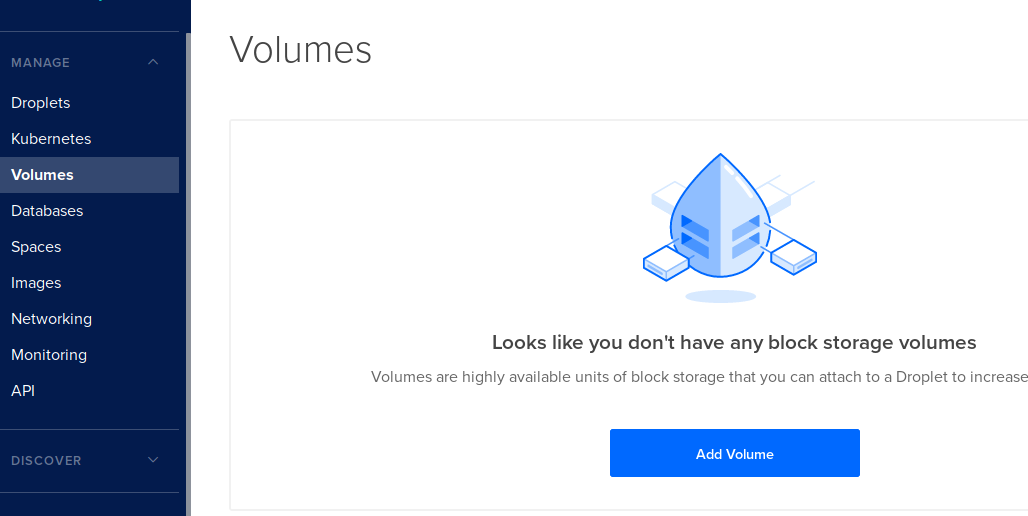
\includegraphics[width=0.95\textwidth]{Images/00_addVolume.png}
\end{center}

\subsection{Add a Tiny Volume for Swap Space}
\begin{center}
   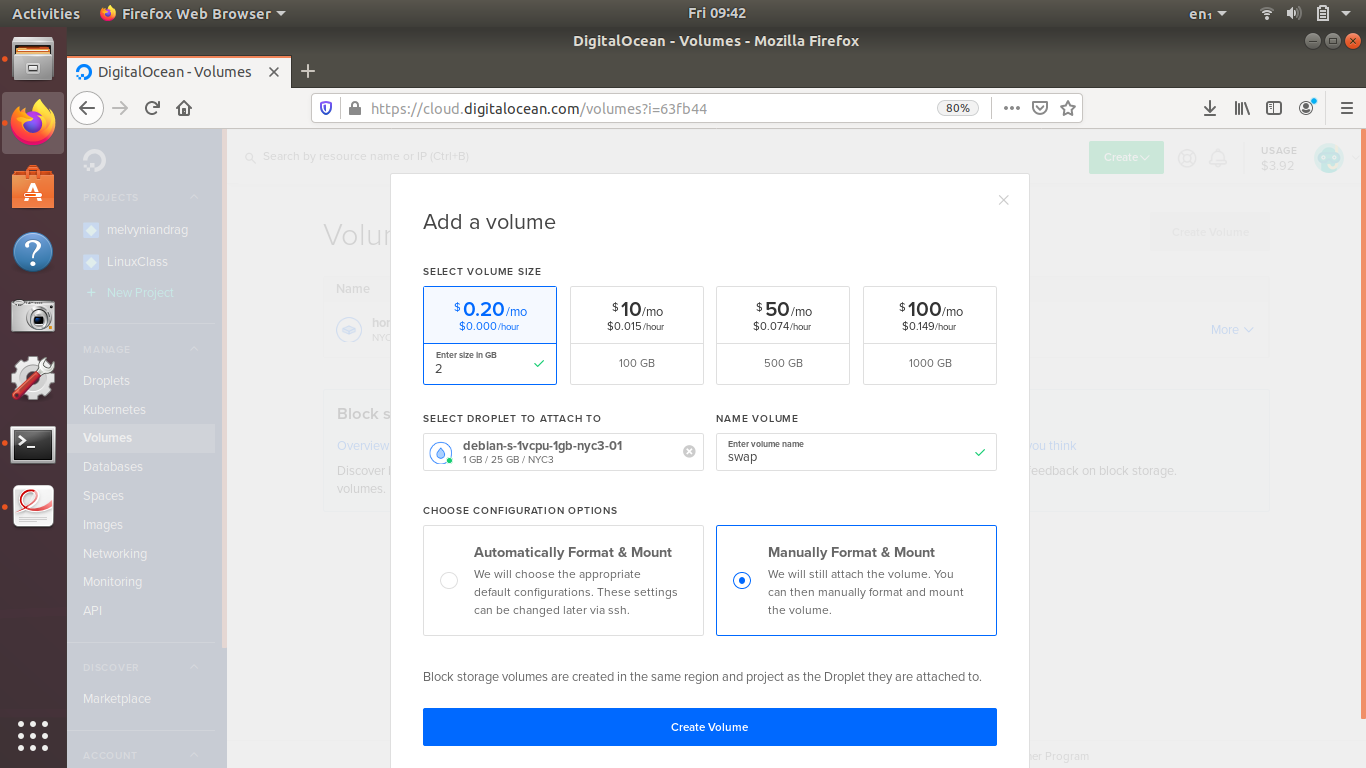
\includegraphics[width=0.95\textwidth]{Images/01_addSwapVolume.png}
\end{center}

\subsection{Add a Tiny Volume for \textit{/home}}
\begin{center}
    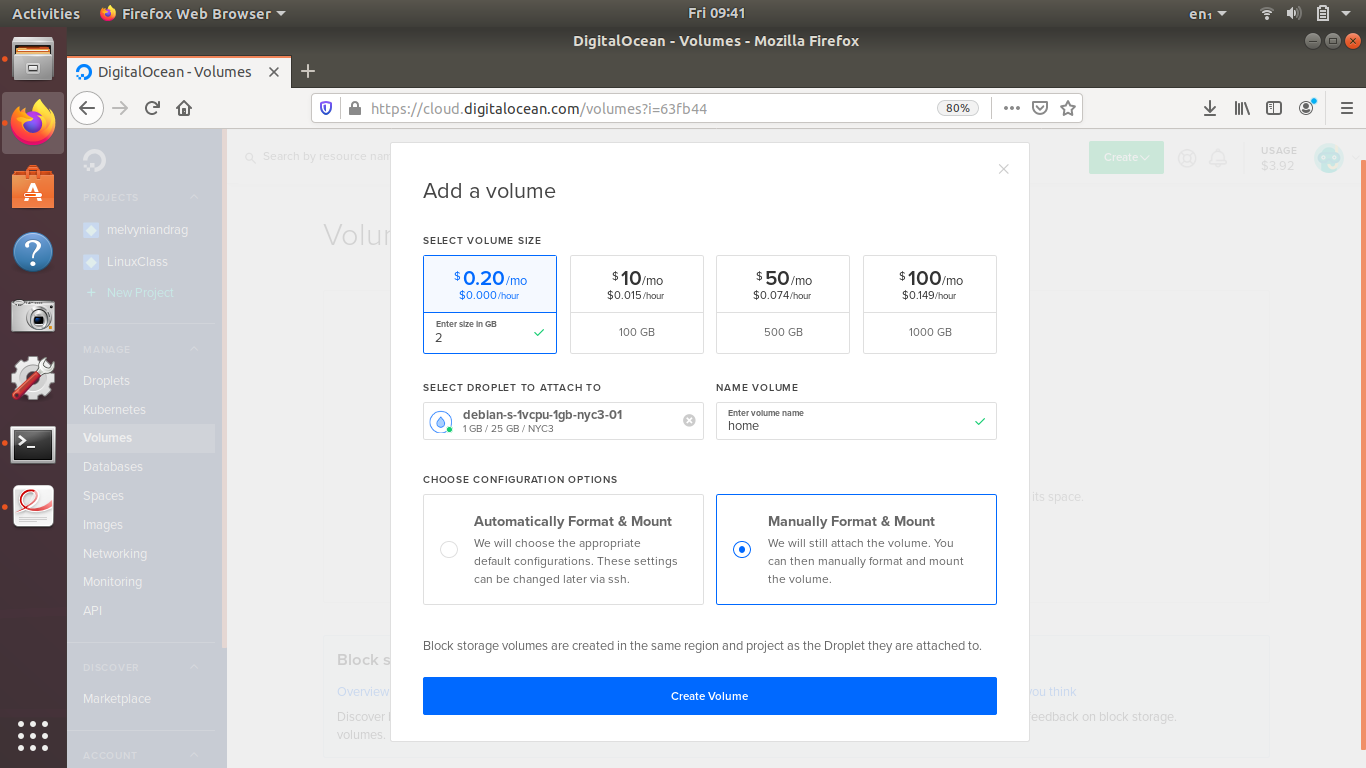
\includegraphics[width=0.95\textwidth]{Images/02_createVolumeHome.png}
\end{center}

\subsection{Make Sure You Have Two Disks}
\begin{center}
    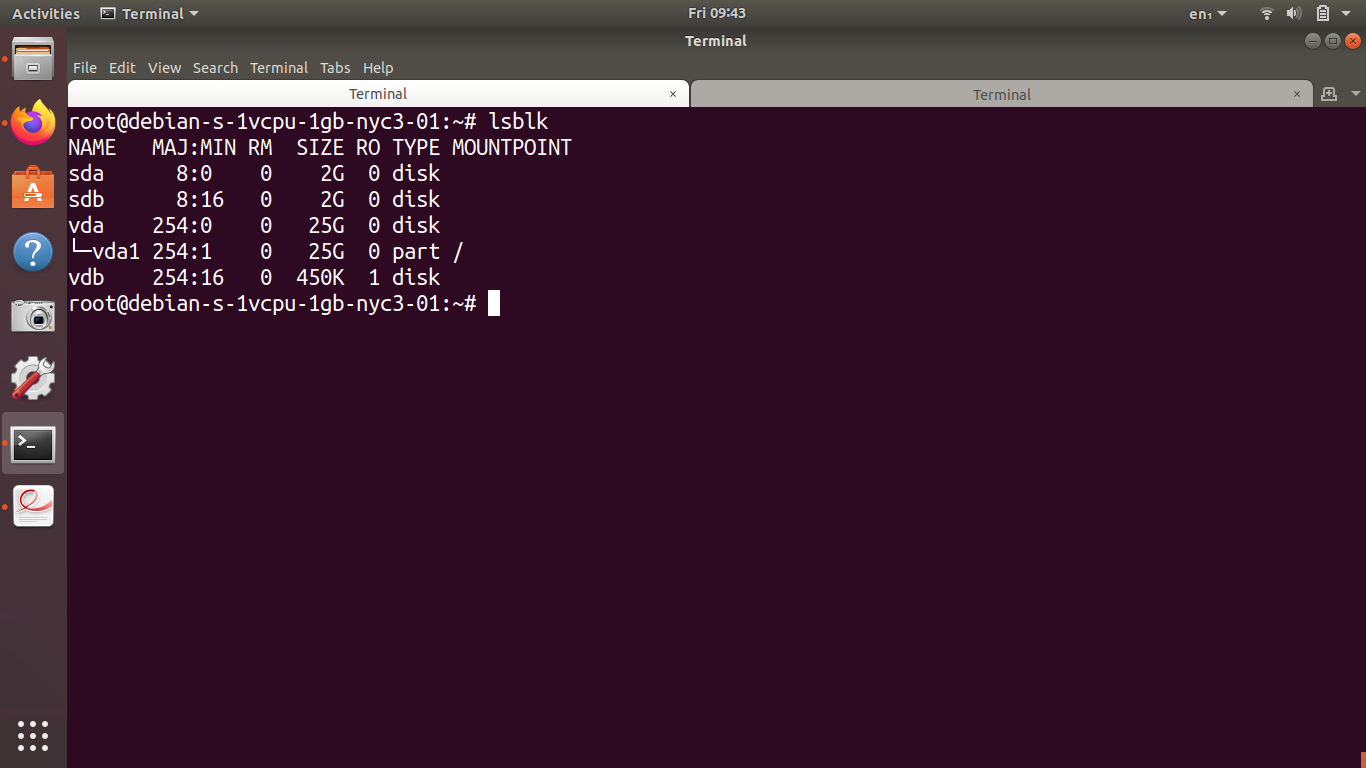
\includegraphics[width=0.95\textwidth]{Images/03_haveTwoDisks.png}
	\textit{Note I have disks /dev/sda and /dev/sdb in my \textbf{lsblk}
results. Those are the two disks added in the previous step.}
\end{center}

\subsection{Format one disk for \textit{/home}}
\begin{center}
    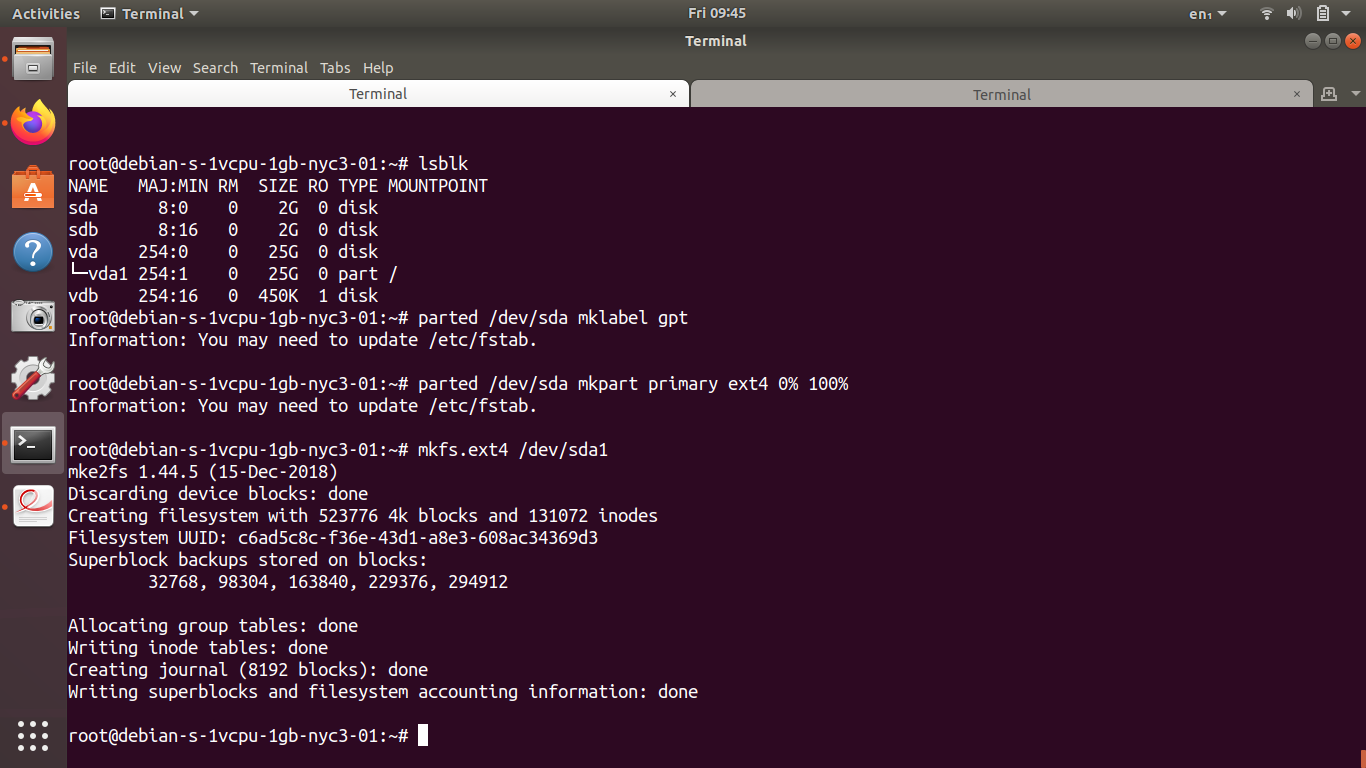
\includegraphics[width=0.95\textwidth]{Images/04_formattedDiskForHome.png}
	\textit{I chose to use /dev/sda for my home partition. It makes no difference
which you chose.}
\end{center}

\subsection{Format one disk for swap space}
\begin{center}
    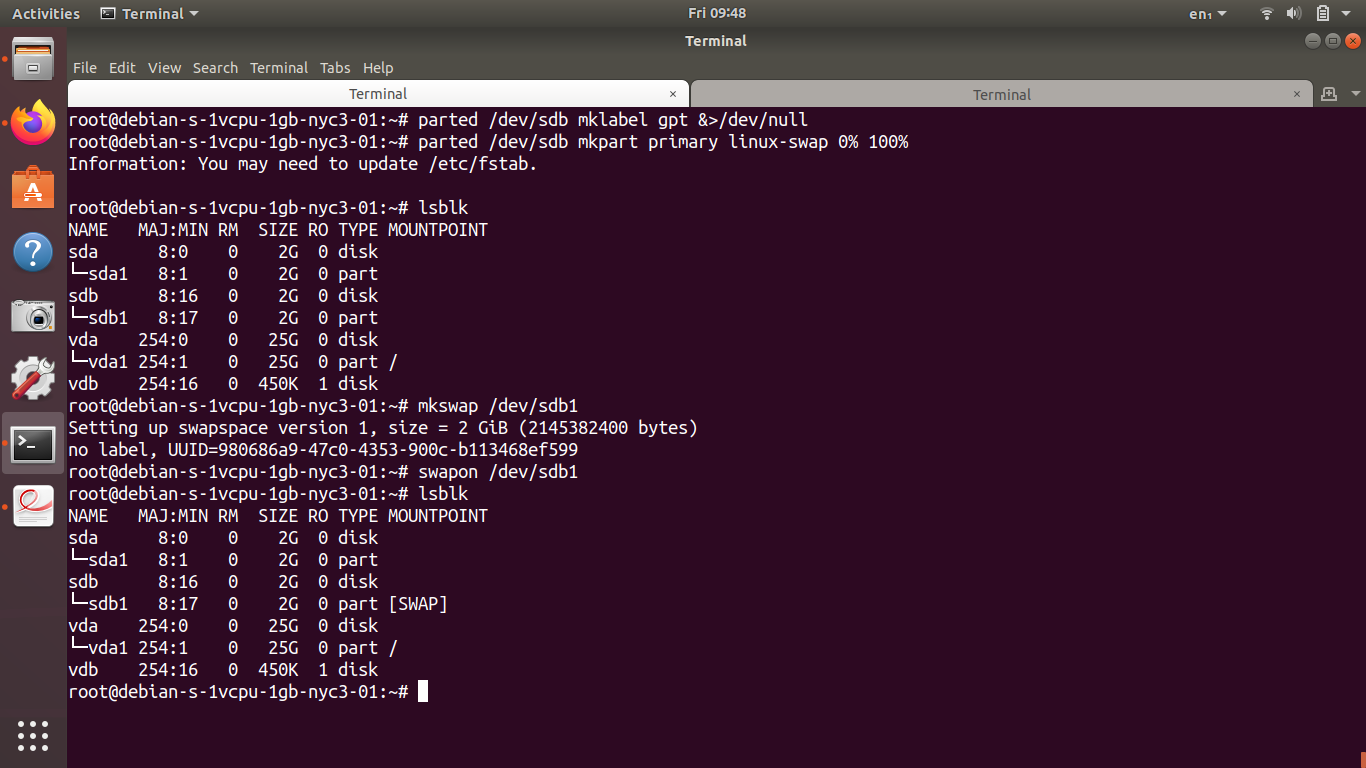
\includegraphics[width=0.95\textwidth]{Images/05_formattedForSwap.png}
	\textit{Format /dev/sdb for swap space and turn swap on so you can verify it
worked.}
\end{center}

\subsection{Modify \textit{/etc/fstab}}
\begin{center}
    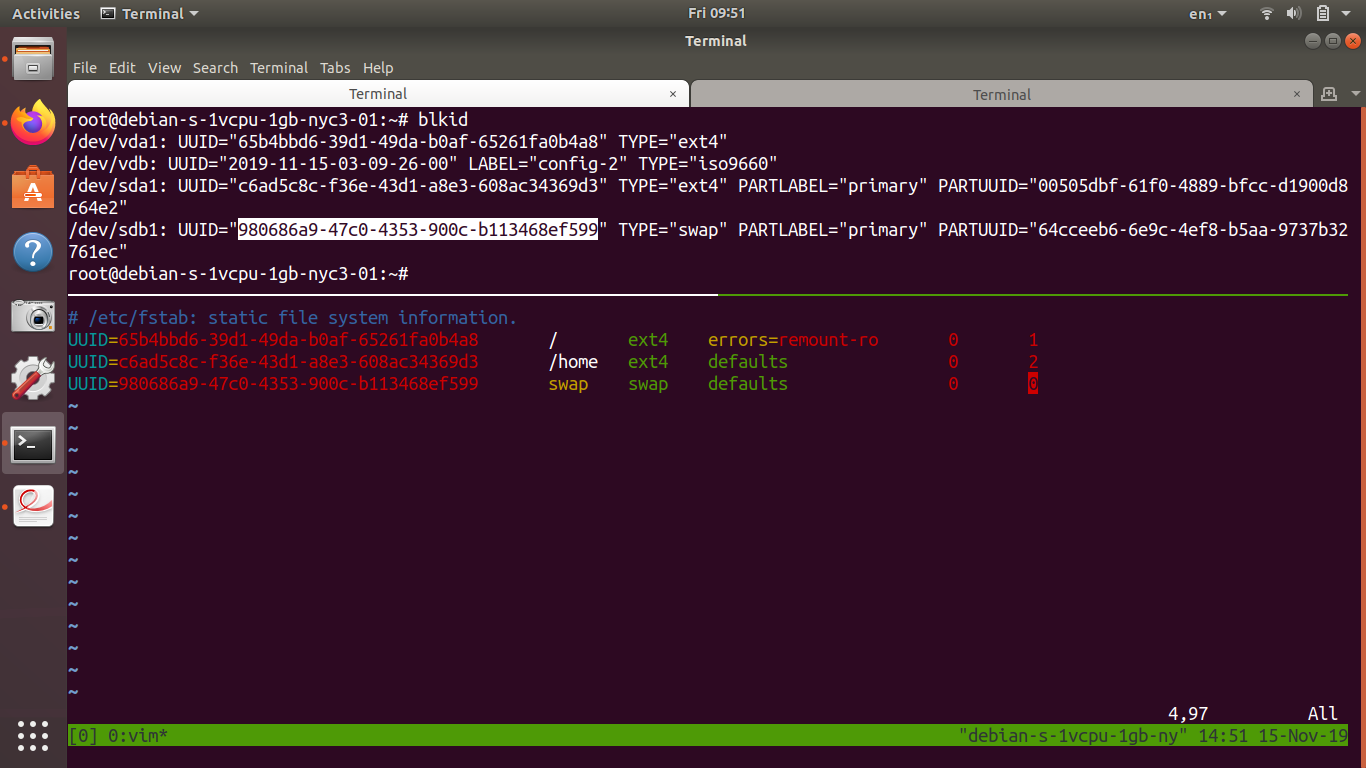
\includegraphics[width=0.95\textwidth]{Images/06_fstab.png}
	\textit{Edit /etc/fstab so that the new disks are mounted on reboot. Pay
careful attention to the contents of this file - we already saw in class how a
typo can be catastrophic!}
\end{center}

\subsection{To be thorough, lets add a user ( so \textit{/home} isn't empty )}
\begin{center}
    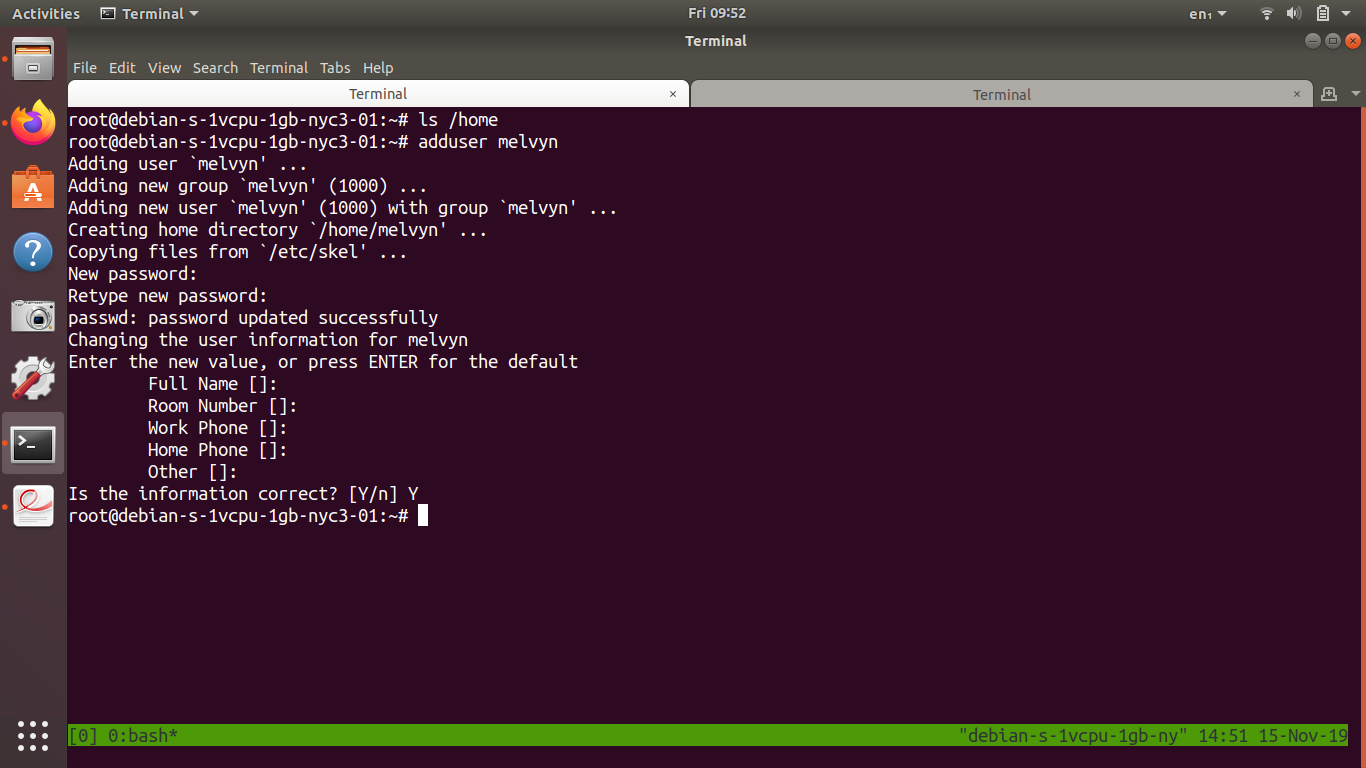
\includegraphics[width=0.95\textwidth]{Images/07_addUser.png}
	\textit{/home is empty. Let's add a user so there's some stuff in /home.}
\end{center}

\subsection{Let's add one more user for good measure}
\begin{center}
    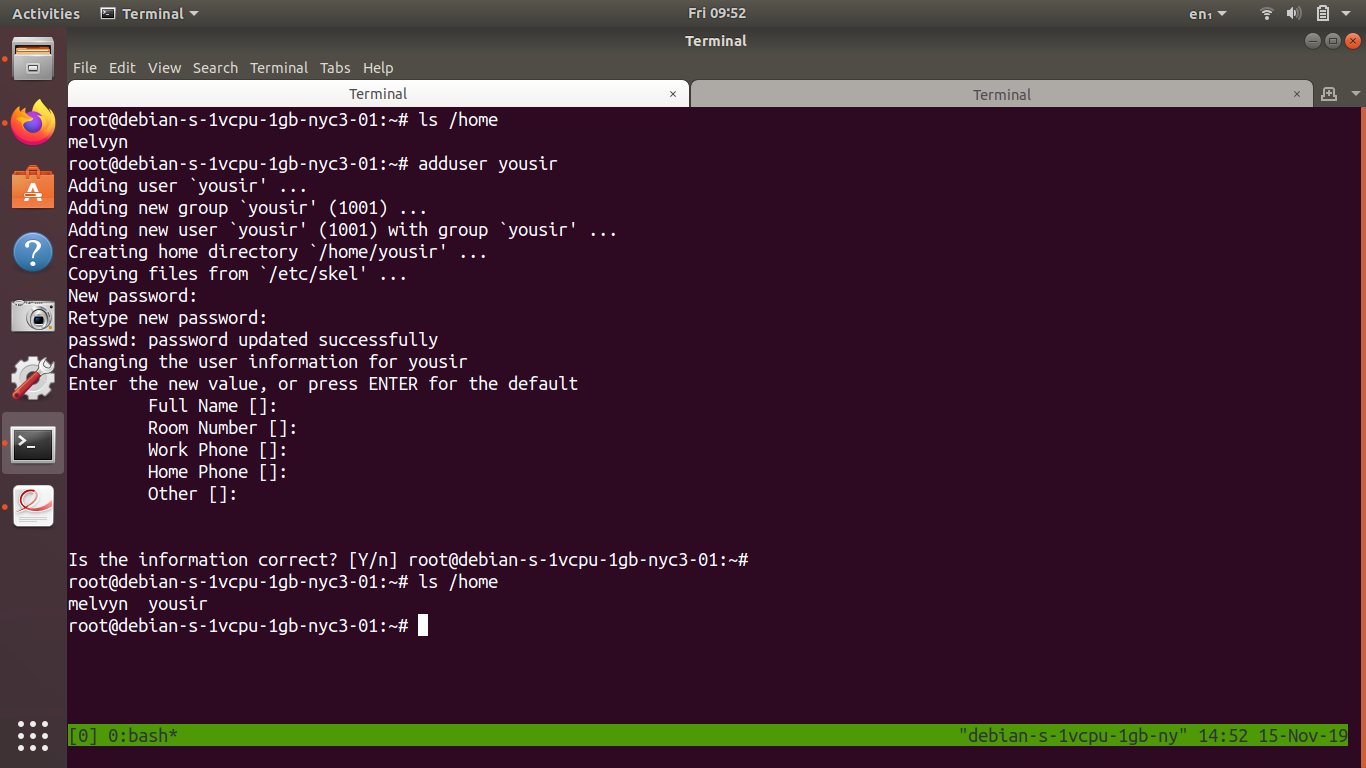
\includegraphics[width=0.95\textwidth]{Images/08_addUser.png}
	\textit{Kind of boring to add just one user. Let's add another one so /home
has two users' home directories.}
\end{center}

\subsection{Have a peek at \textit{/home} permissions before moving to new disk}
\begin{center}
    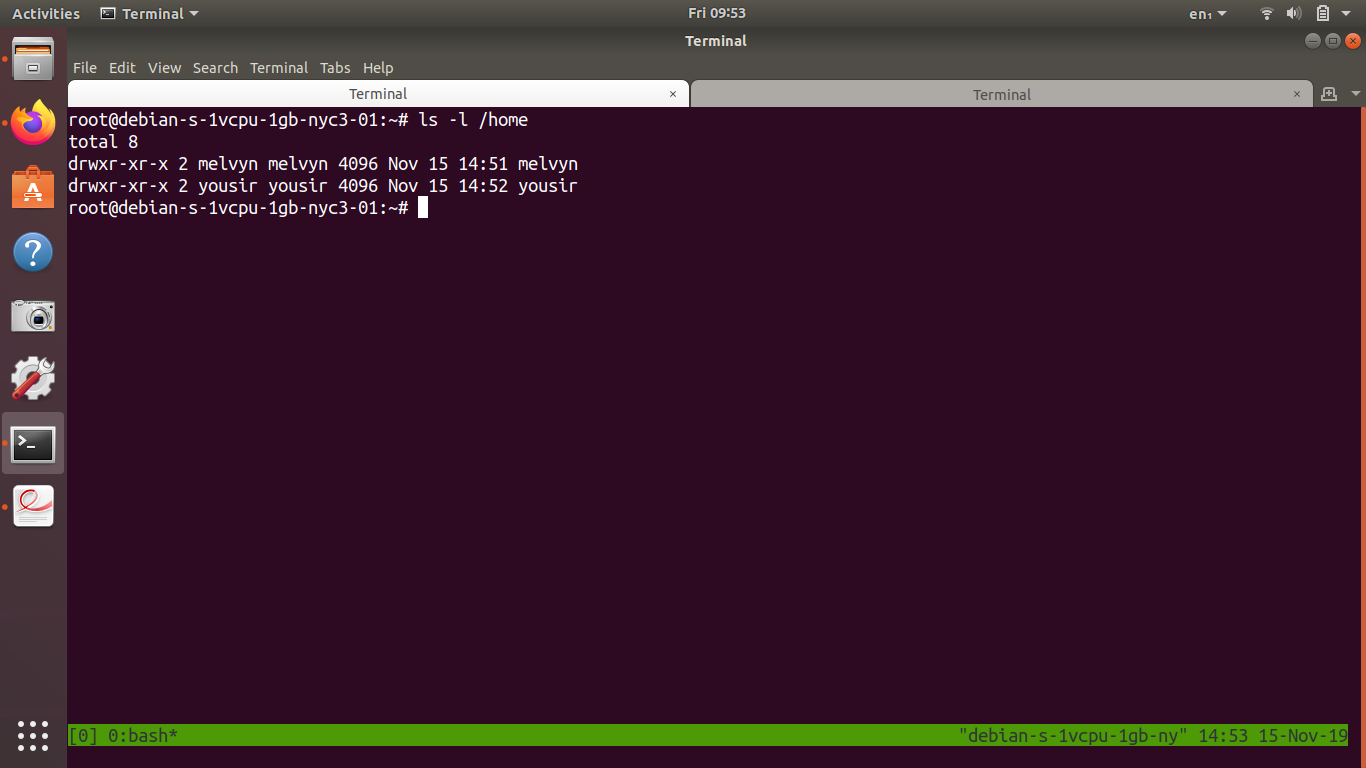
\includegraphics[width=0.95\textwidth]{Images/09_homePermissions.png}
	\textit{Now /home is more interesting.}
\end{center}

\subsection{Move \textit{/home} and verify permissions are still correct.}
\begin{center}
    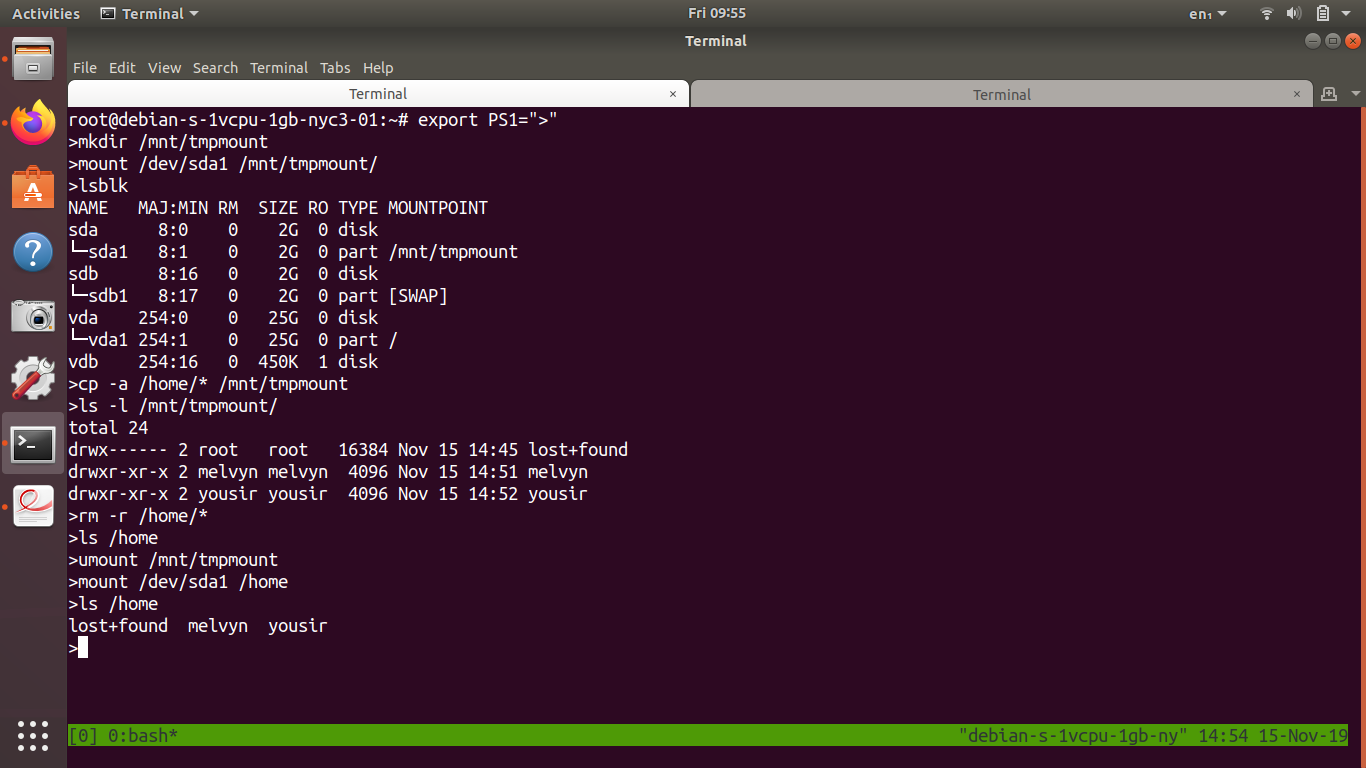
\includegraphics[width=0.95\textwidth]{Images/10_successfullyMovedHome.png}
	\textit{Move the home directory to the new partition. Just take a quick peek
to see that the move went successfully.}
\end{center}

\subsection{Reboot and verify that the swap space and home partition are still
mounted}
\begin{center}
    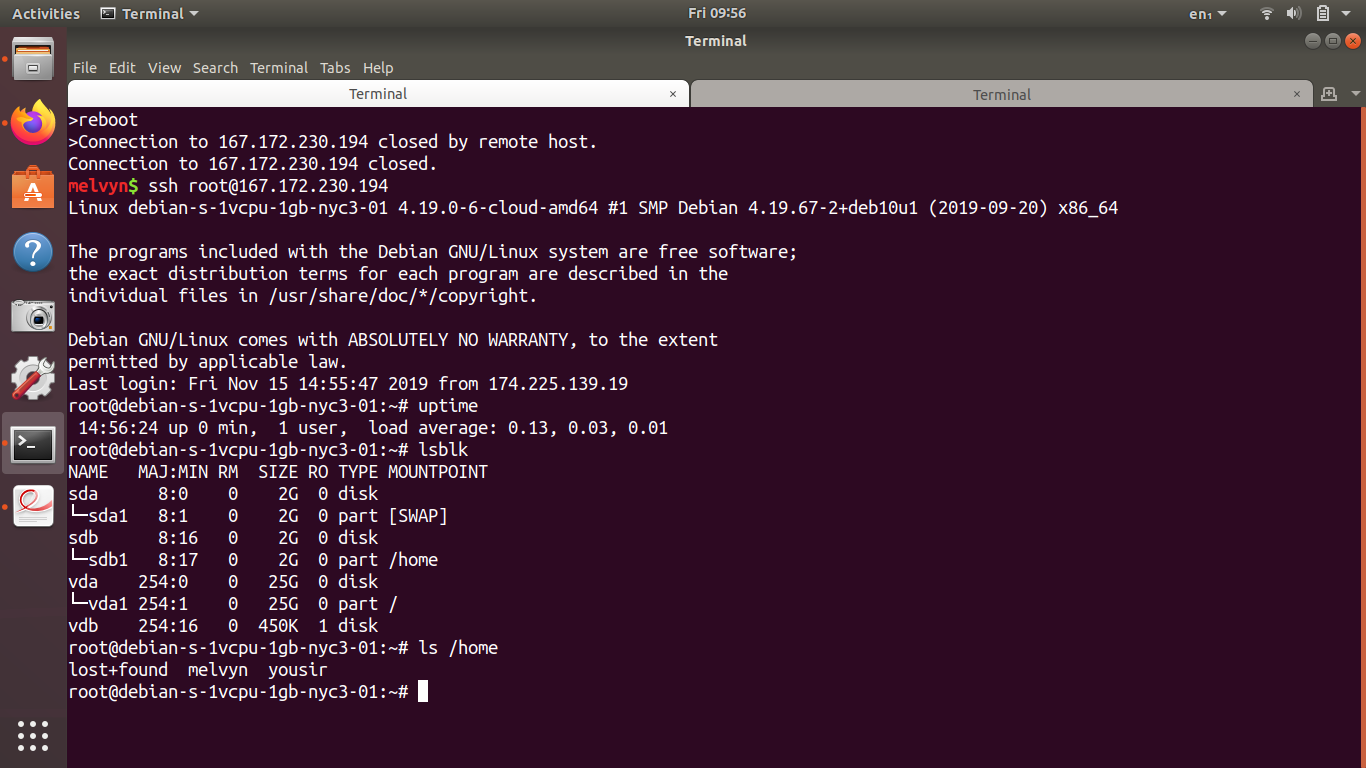
\includegraphics[width=0.95\textwidth]{Images/11_done.png}
	\newline\textit{voila! It worked! Note that now /dev/sda1 is the swap
partition and /dev/sdb1 is the /home partition. This is because sda1 and sdb1
are \textbf{NOT PERSISENT NAMES}. This is why we refer to our disks by their
UUIDs in /etc/fstab instead of referring to disks by their names /dev/sdX}
\end{center}


\section{References} Follow these excellent online tutorials.: 1.
https://linuxize.com/post/how-to-add-swap-space-on-debian-9/ 2.
https://opensource.com/article/18/9/swap-space-linux-systems

\end{document}
